\documentclass[twoside,10.5pt]{article}
\usepackage{jmlr2e}
\usepackage{subfigure}
\usepackage{hyperref}
\usepackage{endnotes}
\usepackage{enumitem}
\setlength{\parskip}{0pt}
\setlength{\parsep}{0pt}
\setlength{\headsep}{5pt}
\setlength{\topskip}{0pt}
\setlength{\topmargin}{0pt}
\setlength{\topsep}{0pt}
\setlength{\partopsep}{0pt}
\let\footnote=\endnote
\renewcommand{\notesname}{Endnotes}
\newcommand{\dataset}{{\cal D}}
\newcommand{\fracpartial}[2]{\frac{\partial #1}{\partial  #2}}
\ShortHeadings{95-845: AAMLP Proposal}{Gangwar, Rost and Setia}
\firstpageno{1}

\begin{document}

\title{Heinz 95-845: Project Report}

\author{\name Mridul Gangwar \email mgangwar@andrew.cmu.edu \\
       \addr Heinz College of Information Systems and Public Policy\\
       Carnegie Mellon University, Pittsburgh, PA, United States \
       \AND
       \name Lauren Rost \email lrost@andrew.cmu.edu \\
       \addr Heinz College of Information Systems and Public Policy\\
       Carnegie Mellon University, Pittsburgh, PA, United States \
       \AND
       \name Nikita Setia \email nikitas@andrew.cmu.edu \\
       \addr Heinz College of Information Systems and Public Policy\\
       Carnegie Mellon University, Pittsburgh, PA, United States}
       
\maketitle
\vspace*{5px}
\begin{abstract}
Opioid overdose deaths spiked in 2017, continuing to be a major concern for the US healthcare system. Major efforts have been dedicated to understand the demographic impacted and how the healthcare system can improve outcomes for individuals at risk. This paper explores the application of machine learning and statistical analyses to identify which could best predict (and prevent) overdose deaths using county-provided demographic, program activity and opiate prescription fills data for Medicaid beneficiaries from 2009-2017. The most superior models, Logistic Regression and Random Forest, yield an AUROC of approximately 85\%, correctly identifying 57\% of individuals who overdose. *Need to add a line about variable importance*. As such, this paper showcases how county-provided data can be used to predict and prevent overdoses (translatable to other counties), identifies the variables indicative of risk, and highlights modeling techniques that can be tuned to improve predictive performance, thereby taking a giant step towards overdose prevention.  
\end{abstract}

\section{Introduction}
Opioid abuse has been an emerging public health issue, and was declared a Public Health Emergency in 2017\footnote{\cite{HHS}}. National drug overdose deaths have increased over the past two decades, from 16,849 in 1999 to 70,237 in 2017\footnote{\cite{NIDA_ODR}}. This trend is especially affected by the onset of the opioid epidemic in the late 1990s\footnote{\cite{NIDA_OOC}}. Approximately 67\% of the overdose deaths in 2017 are due to involvement of any opioids and 24\% are specifically due to prescription opioids \footnote{\cite{NIDA_ODR}}. It has become pertinent, now more than ever before, to better understand the risk factors leading to overdoses and to determine the best way to prevent overdose deaths. \\

Crosier et al. predicted overdose frequency using random forests in order to uncover important features related to overdose frequency and course\footnote{\cite{Sage}}. Lobo et al. identified sub-groups of Pennsylvania patients at greater risk for opioid abuse in a k-means clustering algorithm\footnote{\cite{Lobo}}. This paper aims to contribute to this existing body of work by identifying data variables that are most indicative of risk, which could be crucial to preventing addiction and overdoses. In 2005, the Opioid Risk Tool was developed to help flag patients at risk for opioid abuse and overdose\footnote{\cite{Webster}}. However, due to the subjective nature of this tool and the spike of deaths in 2017, machine learning has been sought to provide a more objective and quantitative approach to estimate risk of opioid abuse and overdose. Acion et al. used a super learning approach to predict the successful treatment for patients with substance use disorders\footnote{\cite{Acion}}. Haller et al. utilized natural language processing on electronic health record data to assess risk and predict opioid abuse \footnote{\cite{Haller}}. \\

This paper strives to expand upon the aforementioned previous work, by identifying the machine learning algorithms that yield the highest predictive performance. Specifically, those models that correctly identify the greatest number of at-risk individuals. This project uses a set of demographic features, usage of county-provided programs, and opioid prescription information to predict overdose deaths (opioid and non-opioid). Specifically, it analyzes the data of Medicaid beneficiaries from 2009 to 2017 provided by Allegheny County Department of Human Services (DHS) to predict the risk of an individual dying due to an non-opioid or opioid-related overdose. The likely outcome of this analysis is the finding of at least one feature and at least one machine learning technique that is highly deterministic in the prediction of overdose deaths, thereby enhancing the space of addiction and overdose death prevention. 

\section{Methods}
\subsection{Original Data Description}
DHS provided 3 datasets: demographic, program activity, and opiate prescription fills. These provide information for 120,650 individuals who have utilized DHS services between 2009 and 2017. The demographic dataset contains the following variables: person ID, race and gender. Figure \ref{fig:orig_dem} in the appendix displays the summary of the demographic dataset. Two points to note are: first, there are 19,531 individuals with no reported race and 210 individuals with no reported gender; second, there is also only one individual who is transgendered male to female and only 19 individuals who are Native Hawaiian / Pacific Islanders. \\

Figure \ref{fig:orig_prog} in the appendix summarizes the original program activity data. The program dataset contains 2,402,479 rows as each row is recording the activity (or activities) for an individual in any year-month since they entered the system. It contains the following variables: person ID, year and month of activity, the relevant activity information, and overdose details, if any. The program-related activity information collected includes: whether CYF program was used as child or parent (binary), the number of criminal court cases (drug or not) filed, whether mental health, drug and alcohol abuse, or prescription service was used (binary), and whether the individual was jailed (binary). Note that if an individual did not overdose, then those variables contained no information for said individual. Else, it was a 0 for non-opiate overdose and 1 for an opiate overdose. As such, this missingness is meaningful. There appears to be no additional missing data in the program activity dataset. \\

Figure \ref{fig:orig_presc} in the appendix showcases the prescription data summary. This dataset contains 1,161,650 rows as each row is a prescription fill for an individual. The prescription information provided includes: the claim number (unique for each row), person ID, age at prescription, dispensed quantity, days supply, fill date, and information specific to the drug (drug strength, name variations, package description, and dosage form). Some points of note are: first, the last two columns (i.e. generic tier description and claim rank) provide no additional information and can be disregarded; second, there are missing, extreme or incomprehensible values in the prescription dataset, such as an age of -7990, dispensed quantity of 17936 and days supply of 907; third, there are three columns containing the drug names which all contain multiple name versions of the same drug; last, there are two columns pertaining to the dosage form, a condensed version and a descriptive version.

\subsection{Data Cleaning and Feature Extraction}
\subsubsection{Demographic and Program Datasets}
The missing race and gender information in the demographic dataset is possibly missing not at random (MNAR) as it may be directly related to the unreported value itself. So, this missingness was dealt with by allowing it to be its own category. Furthermore, in the race column specifically, given that the "Native Hawaiian / Pacific Islander" category was too small it was merged with the "No Data" category to create a new category called "No Data and Other." This was replicated for the gender column, merging the "Transgendered male to female" and the "No Data" categories into "No Data and Other."  In the program activity dataset, the outcome variable was cleaned by converting the 0, 1 and NA to "Non-Opiate Overdose", "Opiate Overdose" and "No Overdose". 

\subsubsection{Opiate Prescription Fills Dataset}
Here are the cleaning tasks performed on this dataset:
\begin{enumerate}[topsep=0pt,itemsep=-1ex,partopsep=1ex,parsep=1ex]
  \item Extracted the age at which an individual got their first prescription (entered the dataset). If the minimum age was less than 0, the maximum age was used. If both values were less than 0, then they were considered missing. There were 26 individuals with missing age values; these were replaced with the median age of individuals in the entire dataset
  \item Updated drug strength values: of oral solutions to 5-325/5ML and of Naloxone to 50MG-0.5MG
  \item Cleaned days supply and dispensed quantity by censoring the extreme values. The top extreme values were replaced with the value at the 0.5\% percentile and bottom extreme with the value at the 95.5\% percentile. These percentile values were determined for each generic name and dosage form combination. 
  \item Pulled opioid strength values from the drug's label name, normalized to be per 1 ML, MCG or MG (if applicable). Replaced missing values with those from provided drug strength column. 
  \item Obtained Opioid Morphine Equivalent Conversion Factors\footnote{\cite{CMS}} to convert the above-mentioned opioid strength values into Morphine Milligram Equivalent (MME). The formula used is: 
  $opioid\,strength * (dispensed\,quantity / days\,supply) * conversion\,factor$
  \item Stripped the drug name (generic name) down to a common terminology to lower the number of categories. For example, "Oxycodone HCL" was replaced with "Oxycodone."
  \item Replaced dosage forms with common terminology to reduce the number of categories. For example, "Tablet" and "Capsule" were changed to "Pill."
\end{enumerate}

\subsubsection{Final Dataset}
30 meaningful features were extracted at the person ID level regarding each individual's demographic characteristics, their participation in DHS program activities, and their opiate prescription fills. Demographic characteristic features include: race, gender and age. DHS program usage features entail: cohort i.e. the start year, usage of CYF program as child ($total\_cyfchild$) and as parent ($total\_cyfparent$), use of mental health, drug and alcohol abuse and prescription services ($total\_mh$, $total\_da$, $total\_rx$), number of months spent in jail ($total\_acj$), and number of criminal cases ($total\_cr\_cases$) and drug-related cases filed in court ($total\_cr\_drug\_cases$). \\

Prescription activity features extracted include: the number of prescriptions ($num\_presc$), name of the most prescribed drug ($most\_presc\_drug$) and most prescribed dosage form ($most\_dose\_form$), count of top three drugs ($oxy\_count$, $tram\_count$, $hydrobit\_count$), count of top three dose forms ($pill\_count$, $patch\_count$, $liquid\_count$), average, median and mode MME ($avg\_mme$, $median\_mme$, $mode\_mme$), as well as average days supply and dispensed quantity ($avg\_supply$ and $avg\_dispensed$). Finally, overdose information ($od\_type$, $od\_month$, $od\_year$, $od\_date$) was added. 

\subsubsection{Feature Choices}
Some additional feature choices were made to enhance the final dataset and prepare for the prediction tasks. Features such as $most\_presc\_drug$ and $most\_dose\_form$, had categories that comprised less than 0.2\% of the values. To prevent errors during the prediction task, these low occurrence categories were combined to create a separate “Other” category. Plotting the distribution of the average, median and mode MME variables revealed that the median MME is less skewed and approximately normally distributed. Therefore, only the median MME was retained in the final dataset to avoid multicollinearity.\\

The target or outcome variable was set to binary with 1 for Opiate Overdose or Non-Opiate Overdose and 0 for No Overdose. Non-opiate overdose simply means that no opioids were found in the individual's system upon death; however, given that these individuals were getting opioid prescriptions and they did overdose, they were included as 1 in the target variable. Furthermore, an argument could be made that individuals who overdose (opiate or non) share similar characteristics and so the additional data would be useful for the prediction task.\\ 

Columns pertaining to the date of overdose were removed to avoid leakage in the machine learning models, as they are proxies for the target variable. All categorical variables were converted to dummy variables. Furthermore, a log transformation was applied to all variables prior to appending the target variable. 

\subsection{Cohort}
Table \ref{tab:table1} below provides an overview of the 120,650 individuals in the Allegheny County DHS cohort between 2009 and 2017. No individuals were excluded from the cohort. All missingness has been addressed to the extent possible; the strategy to address missingness as well as the assumptions made have been clearly stated.

\begin{table}[h!]
  \begin{center}
    \caption{Demographics of Allegheny County DHS Cohort (2009-2017).}
    \label{tab:table1}
    \begin{tabular}{l|c|r} % <-- Alignments: 1st column left, 2nd middle and 3rd right, with vertical lines in between
      \textbf{Characteristic} & \textbf{N} & \textbf{Percentage (\%)}\\
      \hline
      $Race$ & $ $ & $ $ \\
      White & 56,754 & 47.04\\
      Black/African-American & 40,573 & 33.63\\
      Biracial/Multiracial & 2,118 & 1.75\\
      Asian & 1,216 & 1.00\\
      American Indian/Alaskan Native & 439 & 0.36\\
      No Data and Other & 19,550 & 16.20\\
      \textbf{Total} & \textbf{120,650} & \textbf{100}\\
      \hline
      $Gender$ & $ $ & $ $ \\
      Female & 73,582 & 60.99\\
      Male & 46,857 & 38.84\\
      No Data and Other & 211 & 0.17\\
      \textbf{Total} & \textbf{120,650} & \textbf{100}\\
      \hline
      $Age (years)$ & $ $ & $ $\\
      0-19 & 27,128 & 22.48\\
      20-39 & 51,883 & 43.00\\
      40-59 & 35,941 &  29.79\\
      60 \& Over & 5,698 &   4.72\\
      \textbf{Total} & \textbf{120,650} & \textbf{100}\\
      \hline
    \end{tabular}
  \end{center}
\end{table}

%%%Do we add anything else here?? any other EDA??

\subsection{Models}
This paper explores and compares five machine learning models in their performance in predicting whether an individual will overdose. These models are multivariate logistic regression, ridge regression, random forest, ada boosting, and gradient boosting. 

Please add details regarding the machine learning models... also add a subsubsection pertaining to oversampling.

\subsection{Evaluation Criteria}
Need to explain AUROC, accuracy and other criteria we used to evaluate.
Need to note that will also be striving to purely understand probability of survival and see if varies across subgroups (race, gender). Also, will be looking at importance of variables across models (rf, lr, survival). These are not necessarily evaluating these models, but allowing us to compare them and noting them for future work to compare as well. 

\section{Results}

\subsection{AUROC}
We ran a series of machine learning methods to predict overdose deaths. We were not able to detect sufficient overdose deaths with logistic regression, and thus we implemented an oversampling method, Synthetic Minority Oversampling Technique (SMOTE). This gave us a AUC of 0.85. 
We ran multivariate logistic regression on selected features using 5-fold cross-validation.
We then ran ridge regression using lasso regularization and 10-fold cross-validation.
We also applied random forest to predict overdose death, also using 10-fold cross-validation. 
Gradient boosting machine with 10-fold cross-validation led to an AUC of 0.85.
AdaBoost gave poorer performance than the aforementioned methods, with an AUC of 0.75. We then tested the performance of a neural network to predict opioid death, and found an even lower AUC of 0.5, equal to chance. 

\begin{figure}[htp]
\centering
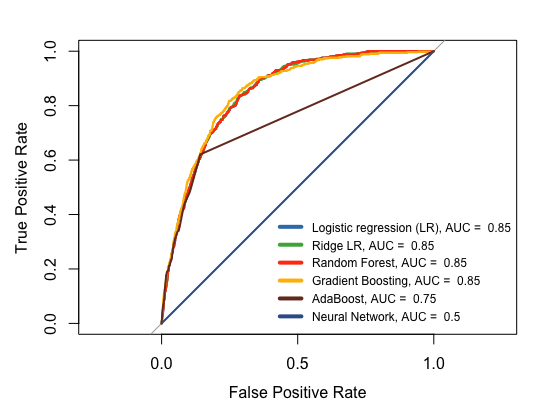
\includegraphics[width=12cm]{images/AUC_ML_opioids.png}
\caption{Predictive performance for overdose deaths had an AUC of 0.85 for three machine learning methods (logistic regression, ridge logistic regression, and random forest), but demonstrated poor performance for gradient boosting, AdaBoost, and neural network).}
\label{fig:lion}
\end{figure}

\subsection{Sensitivity vs. Specificity}

\subsection{Survival Analysis}

\subsection{Variable Importance}


\begin{figure}[htp]
\centering
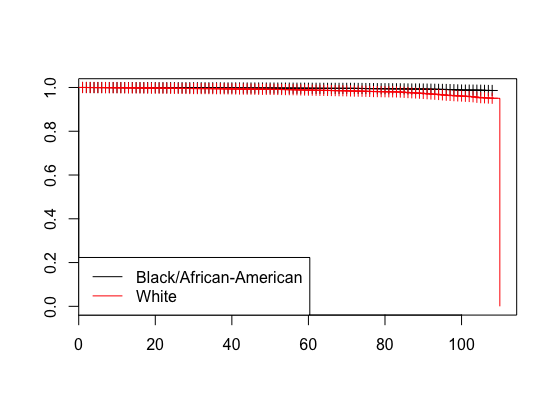
\includegraphics[width=12cm]{images/Race_KaplanMeier.png}
\caption{Kaplan Meier curve of survival indicates that }
\label{fig:lion}
\end{figure}

\begin{figure}[htp]
\centering
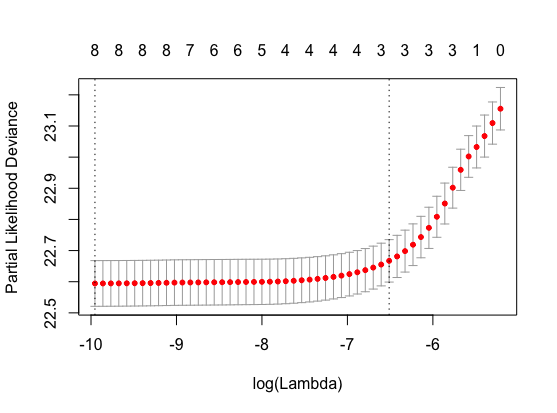
\includegraphics[width=12cm]{images/Coxmodel.png}
\caption{Cox model indicates}
\label{fig:lion}
\end{figure}

\section{Discussion and Related Work}
Significance of results
Limitations 

\section{Conclusion}

\newpage
\appendix
\section*{Appendix A.}
Some more details about those methods, so we can actually replicate them.

We also performed a correlation analysis to better understand the relationship between numerical variables. During the exploration we found out some interesting relationship like hydrobit count is positively correlated with total Rx, number of prescriptions, and pill count.

\begin{figure}
\begin{center}
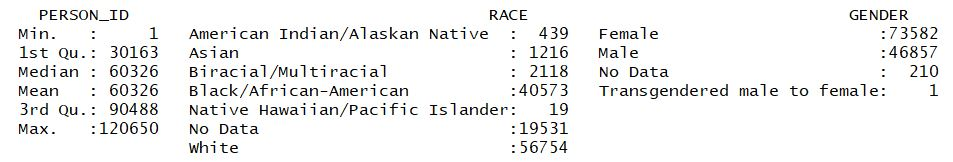
\includegraphics[width=5in]{original_dem_summary.JPG}
\end{center}
\caption{Summary statistics of the original demographic dataset.}
\label{fig:orig_dem}
\end{figure}

\begin{figure}
\begin{center}
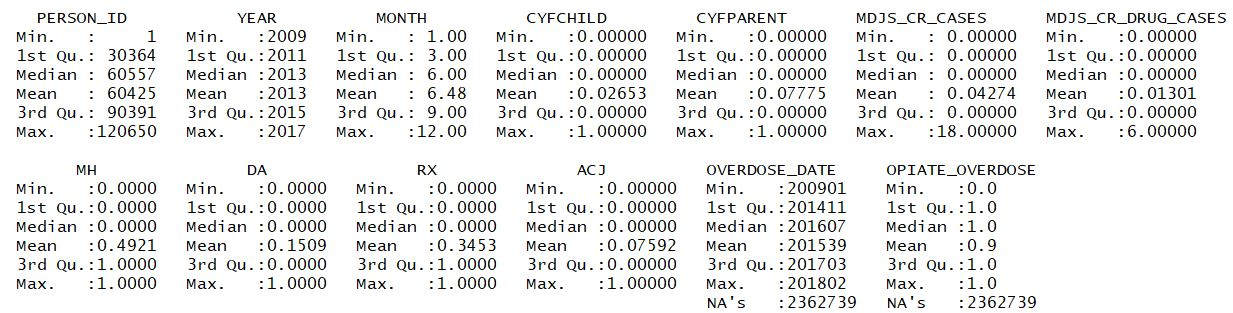
\includegraphics[width=6in]{original_prog_summary.JPG}
\end{center}
\caption{Summary statistics of the original program activity dataset.}
\label{fig:orig_prog}
\end{figure}

\begin{figure}
\begin{center}
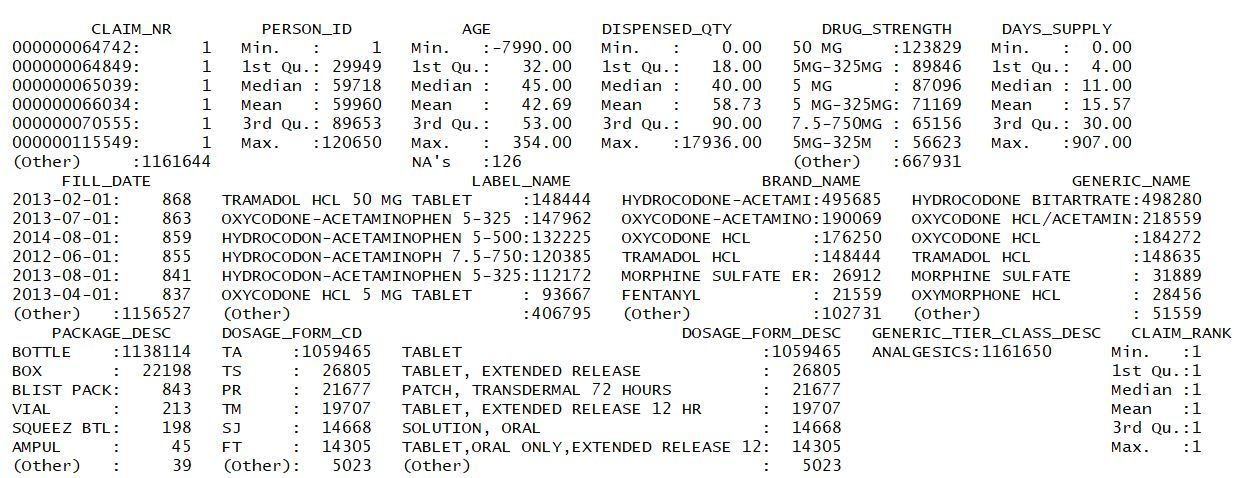
\includegraphics[width=6in]{original_presc_summary.JPG}
\end{center}
\caption{Summary statistics of the original opiate prescription fills dataset.}
\label{fig:orig_presc}
\end{figure}

\newpage
\theendnotes
\bibliographystyle{ieeetr}
\bibliography{final_bibliography.bib}



\end{document} 
